\documentclass[journal]{IEEEtran}
\usepackage[spanish,english]{babel}
\usepackage[T1]{fontenc}
\usepackage{cite}
\usepackage{array}
\usepackage{url}
\usepackage{amsmath}
\usepackage{tikz}
%\usepackage{subfig}
\usepackage{amsfonts}
\usepackage{float}
\usepackage{amssymb}
\usepackage{enumerate}
\usepackage{hyperref}
\usepackage{pstricks}
\usepackage{pictex}
\usepackage{pst-all}
\usepackage{multicol}
\usepackage{booktabs}
\usepackage{siunitx} 
\hyphenation{neo-or-to-do-xia bio-ae-ro-sol}

\begin{document}

\title{Sensor de temperatura con visualización de escala cromática en RGB y escala numérica en monitor conectado por comunicación serial}
\author{Rafael Ricardo Galindo León, Santiago Andrés García Benitez\\
        (rrgalindol, saagarciabe)@unal.edu.co}

\markboth{Sensor de temperatura con visualización en RGB y por monitor}
{Shell \MakeLowercase{\textit{et al.}}: Bare Demo of IEEEtran.cls for IEEE Journals}

\maketitle
\begin{otherlanguage}{english} 
\begin{abstract}
This report corresponds to the development of a Temperature sensor with chromatic and numerical scale, using microcontrollers. The circuit was depeloped with 1 LED RGB for the implementation of the chromatic scale.
\end{abstract}
\begin{IEEEkeywords}
ADC, Arduino, LM35, RGB, Serial Communication, Temperature.
\end{IEEEkeywords}
\end{otherlanguage}
\IEEEpeerreviewmaketitle
\begin{otherlanguage}{spanish}
\section{Introducción}
\IEEEPARstart{H}{a}biendo aprendido y hecho uso de capacidades de los microcontroladores tales como los retardos, las interrupciones, la comunicación serial, entre otros, es posible introducir otra de estas capacidades. La conversión análogo-digital (ADC) es una actividad que resulta de vital importancia en las diversas aplicaciones que se pueden desarrollar con microcontroladores. Esto se debe a que el mundo que nos rodea está construido por variables continuas mientras que las técnicas de almacenamiento y procesamiento de la información, se hace con variables discretas. En una aplicación como el Sensor de temperatura con visualización en RGB y por monitor se pueden evidenciar y poner en práctica y uso la conversión análogo-digital.

\section{Desarrollo}

\subsection{Montaje}
Como primer acercamiento al desarrollo de la práctica, inicialmente se planteó el Diagrama de conexiones del Sensor de Temperatura. Para esto se hizo uso del software KiCad, en el que se realizaron las conexiones respectivas para el LED RGB y el LM35 (sensor de temperatura). A su vez, se planteó la conexión para la comunicación serial teniendo en cuenta el Data Sheet del Microcontrolador. En la Figura \ref{E} se puede observar el planteamiento de la propuesta para el circuito a desarrollar. Teniendo esta primera fase definida, se procedió a realizar el Montaje en Protoboard del Sensor de Temperatura.

\begin{figure}[H]
    \centering
    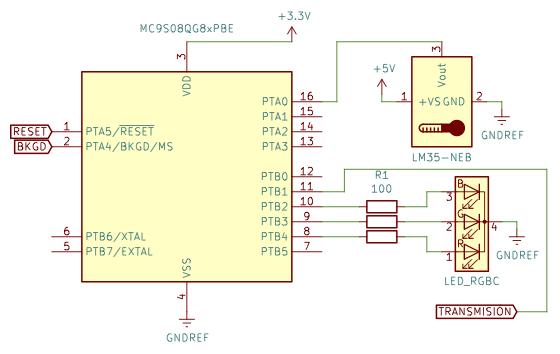
\includegraphics[scale=0.4]{Imágenes/Esquema5.jpg}
    \caption{Esquemático}
    \label{E}
\end{figure}

Para la construcción del Sensor de Temperatura se utilizó el Microcontrolador MC9S08QG8 de la familia HCS08 de Motorola Freescale. A este se conectó un LED RGB a través de resistencias de 100 $\Omega$ y 150 $\Omega$ y un LM35 (sensor de temperatura). El montaje se puede observar en la Figura \ref{M}.

\begin{figure}[H]
    \centering
    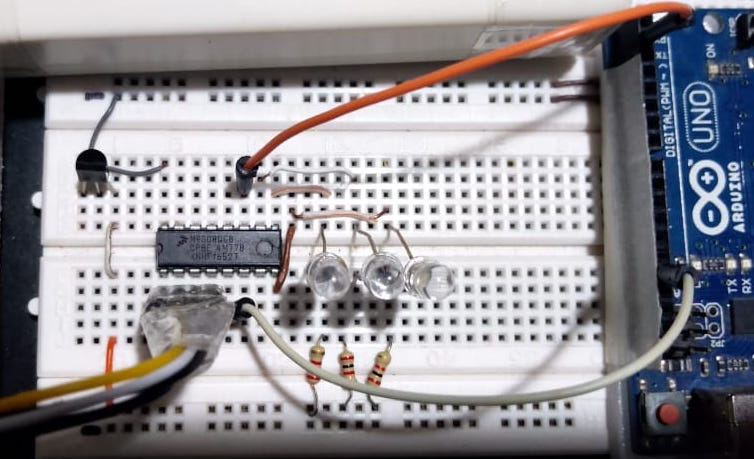
\includegraphics[scale=0.3]{Imágenes/Montaje_Practica_5.jpeg}
    \caption{Montaje en Protoboard}
    \label{M}
\end{figure}

Para la sección del montaje correspondiente a las salidas al LED RGB se designaron los pines PTB0, PTB1 y PTB2 del QG8. A su vez, para la sección correspondiente a la entrada del LM35, el pin PTA0. También se designó el pin PTB1 para la comunicación serial ya que este corresponde al Tx del periférico de comunicación serial diseñado para cumplir la labor de transmisión de datos.

\subsection{Programación}

Para el desarrollo de la lógica del Sensor de Temperatura se utilizó el programa CodeWarrior 10.7. El código se escribió en C.\\

El algoritmo del funcionamiento del Sensor de Temperatura se planteó de la siguiente manera. Se definieron las tareas de: solicitar la medición, realizar un retardo y configurar la salida del LED RGB. A continuación, en la Figura \ref{DDF_General} se presenta el Diagrama de Flujo correspondiente al Contador.

\begin{figure}[H]
    \centering
    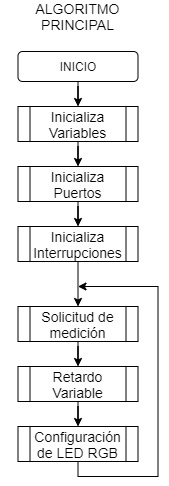
\includegraphics[scale=.52]{Imágenes/Practica 5.1.jpg}
    \caption{Diagrama de Flujo General del algoritmo}
    \label{DDF_General}
\end{figure}

Durante la solicitud de la medición, se realiza una verificación de si la conversión se encuentra en proceso o se ha completado. Lo anterior se hace en el entendimiento de que la conversión toma un tiempo en completarse. Al completarse ese proceso de conversión, se ha obtenido un valor digital. Esta tarea se muestra en la Figura \ref{DDF_MED}.

\begin{figure}[H]
    \centering
    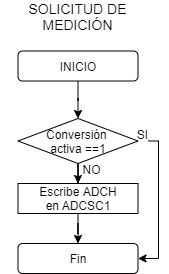
\includegraphics[scale=.52]{Imágenes/Practica 5.2.jpg}
    \caption{Diagrama de Flujo Solicitud de Medición}
    \label{DDF_MED}
\end{figure}

La obtención de un valor digital, luego de haber realizado la conversión, activa una interrupción controlada por el módulo ADC. Para esta interrupción, al igual que las que se han desarrollado en las prácticas anteriores, es importante asegurarse de desactivar la bandera de interrupción de manera que pueda seguir llamándose en el futuro. Esta interrupción activa una nueva lectura e inicia otra conversión de la señal que se está recibiendo. Al hacerlo, guarda el valor obtenido anteriormente en una variable la cual se carga al registro de Data para la Transmisión al monitor. La Figura \ref{DDF_ADC} corresponde al algoritmo de dicha interrupción.

\begin{figure}[H]
    \centering
    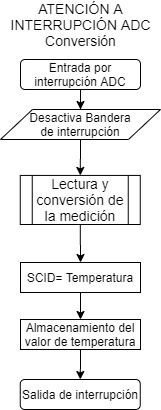
\includegraphics[scale=.6]{Imágenes/Practica 5.6.jpg}
    \caption{Diagrama de Flujo Interrupción Medición Finalizada ADC}
    \label{DDF_ADC}
\end{figure}

Finalmente, se hace la configuración del LED RGB. Esta se hace con un rango de valores para la variable que guarda el valor digital de Temperatura obtenido del módulo ADC. Este rango de valor fue establecido en las condiciones de la aplicación. De esta manera, se tiene:

\begin{table}[H]
        \label{Salidas}
        \centering
        \caption{Código de colores}
        \begin{tabular}{||c||c||c||}
        \hline \hline 
        {\centering \textbf{Temperatura ($^{\circ}$C)}} & {\centering \textbf{Color}} & {\centering \textbf{Código RGB}} \tabularnewline \hline
         T<23 & Negro & 0,0,0 \tabularnewline \hline
         23<T<26 & Azul & 0,0,255 \tabularnewline \hline
         26<T<29 & Cián & 0,255,255 \tabularnewline \hline
         29<T<32 & Verde & 0,255,0 \tabularnewline \hline
         32<T<35 & Amarillo & 255,255,0 \tabularnewline \hline
         35<T<38 & Rojo & 255,0,0 \tabularnewline \hline
         38<T<41 & Magenta & 255,0,255 \tabularnewline \hline
         T<41 & Blanco & 255,255,255\tabularnewline \hline
        \hline 
        \end{tabular}
    \end{table}

Así, se tiene una escala cromática de colores que indican el rango en el que se encuentra la temperatura medida por el LM35 cuyo valor ha sido convertido de análogo a digital por el ADC. La Figura \ref{DDF_RGB} muestra en detalle el algoritmo para esto.

\begin{figure}[H]
    \centering
    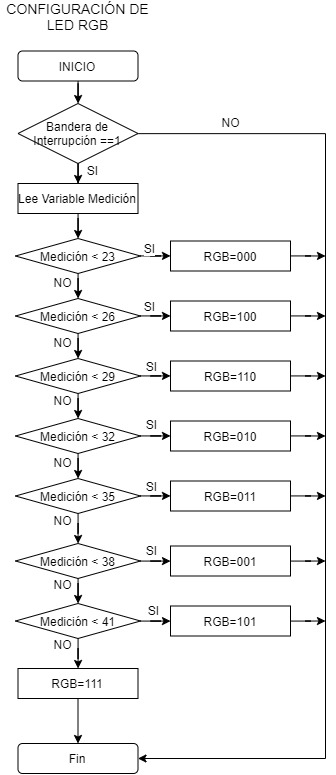
\includegraphics[scale=.5]{Imágenes/Practica 5.3.jpg}
    \caption{Diagrama de Flujo Configuración RGB}
    \label{DDF_RGB}
\end{figure}

\subsection{Comprobación}

En el desarrollo de esta aplicación hubo algunos detalles a tener en cuenta o revisar para asegurar un adecuado funcionamiento. El primero, mencionado también en la práctica anterior, es necesario hacer un adecuado uso de las interrupciones: que se activen en el momento oportuno y se asegure la salida de ellas. En esta aplicación en particular, la interrupción era de vital importancia ya que como la conversión es un proceso que puede ser demorado, no es posible asegurar cuándo se termine. De hacer el programa sin interrupciones, debería ser muy determinista, lo cual aumentaría la complejidad y disminuiría la eficiencia del programa.\\

Justamente, relacionado también con el proceso de conversión, es necesario tener en cuenta dos fenómenos que afectan directamente una aplicación como la desarrollada en esta práctica. Por un lado, es necesario conocer la sensibilidad del sensor que se esté utilizando para la obtención de los datos de entrada. Esto tiene que ver con entender el comportamiento estático y dinámico del mismo, conocer su función de transferencia. Por otro lado, cada microcontrolador tiene una resolución diferente que corresponde a la cantidad de bits que se pueden utilizar para representar el dato obtenido por el conversor. Algunos microcontroladores como el QG8 tienen la posibilidad, incluso, de aumentar de 8 a 10 bits dicha resolución. Tiene que haber un análisis de la correspondencia de la sensibilidad del sensor con la resolución del microcontrolador.\\

Con respecto a la comunicación, al igual que en la práctica anterior, es necesario asegurarse de estar trabajando con el mismo Baud Rate entre el microcontrolador y el Monitor. Así podrá existir comunicación entre los dispositivos. En dicha comunicación vuelve a ser importante asegurarse de que la transmisión de información se realice en su totalidad (implementación de un retardo de transmisión) y, como parte de la información, que los mensajes respectivos se escriban de manera adecuada. Para esto, se hace uso nuevamente de la Tabla ASCII.\\

Por último, cabe mencionar que la aplicación se realizó con LED RGB de Cátodo Común lo anterior para poder manejar una lógica de salida positiva. Sería posible implementarla con un LED RGB de Ánodo Común; lo único es que debería asegurarse de invertir la lógica para así trabajar con lógica de salida negativa. Sin embargo, aunque es posible, no sería necesariamente lo más recomendable ya que la mayoría de documentación con respecto al código RGB se encuentra con lógica positiva y es un estándar que es bueno mantener.


\section{Conclusiones}
\begin{enumerate}
    \item El LM35 es un sensor que complementa muy bien el microcontrolador QG8. Ya que es de bajo costo, resulta muy útil en la fabricación de dispositivo económico. Además, dado que su corriente de alimentación es baja, se puede crear también un dispositivo de bajo consumo, aprovechando a su vez los modos de bajo consumo del microcontrolador.
    \item Como con muchos sensores usados para estas aplicaciones, es importante recordar que dentro de su comportamiento aparentemente lineal, el LM35 puede presentar irregularidades en su comportamiento. Esto puede no necesariamente ser dañino pero sí es necesario tenerlo en cuenta al realizar una evaluación en el funcionamiento de la aplicación.
    \item El proceso para la conversión análogo-digital requiere de tiempo para completarse. Para evitar que la ejecución del programa se vea afectado, se usa una interrupción que se activa cuando se haya finalizado la conversión.
    \item Si se realizara un control de  tensión o ancho de pulso de las salidas conectadas al RGB sería posible generar a una escala con mayor resolución (más variedad de colores, más rangos de temperatura.
\end{enumerate}

\begin{thebibliography}{1ente,5}
    \bibitem{NXP} NXP
    \textit{MC9S08QG8 - MC9S08QG4 Data Sheet.}
    Disponible en: https://www.nxp.com/docs/en/data- sheet/MC9S08QG8.pdf
 
\end{thebibliography}
\end{otherlanguage}
\end{document}